% Foliensatz: "AFu-Kurs nach DJ4UF" von DK0TU, Amateurfunkgruppe der TU Berlin
% Lizenz: CC BY-NC-SA 3.0 de (http://creativecommons.org/licenses/by-nc-sa/3.0/de/)
% Autoren:
% (Martin Deutschmann)
% Sebastian Lange <dl7bst@dk0tu.de>
% Andreas Krüger (DJ3EI) (Dezibel-Erklärung)
% Korrekturen:
% Lars Weiler <dc4lw@darc.de>

\documentclass[aspectratio=169]{beamer}

\usepackage[ngerman]{babel} % deutsche Worttrennung etc.
\usepackage[utf8]{inputenc} % UTF8 Text

\usepackage[super, comma, numbers, square, sort]{natbib}

\usepackage{hyperref}       % Hyperref Package für bessere Referenzen (todo)
\hypersetup{
	colorlinks=false,       %   false: boxed links; true: colored links
    %linkcolor=white,       %   color of internal links (change box color with linkbordercolor)
    citecolor=red,          %   color of links to bibliography
    filecolor=white,        %   color of file links
    urlcolor=blue           %   color of external links
}

\usepackage{multirow}
\usepackage{wasysym}  % Math Symbols like \permil
%\usepackage{colortbl}
%\usepackage{subscript}
%\usepackage{caption}
%\usepackage{setspace}
%\usepackage{xcolor}        % benutze CodeListe

% Footnote
%\usepackage{hanging}
%
%\setbeamertemplate{footnote}{%
%  \hangpara{2em}{1}%
%  \makebox[2em][l]{\insertfootnotemark}\footnotesize\insertfootnotetext\par%
%}


%\usepackage{pgf}
%\usepackage{tikz}
%\usetikzlibrary{arrows,automata}
%\usetikzlibrary{positioning}
%
%\tikzset{
%    state/.style={
%           rectangle,
%           rounded corners,
%           draw=black, very thick,
%           minimum height=2em,
%           minimum width=2pt,
%           inner sep=2pt,
%           text centered,
%           },
%}

%\usepackage{listings}
%\lstset{basicstyle=\small, numberstyle=\tiny, extendedchars=true, numbers=left, numbersep=5pt}
%\lstset{showtabs=false, showspaces=false, showstringspaces=false}
%%\lstset{backgroundcolor=\color{white!75!lightgray}, , frame=single}
%%\lstset{backgroundcolor=\color{white}}
%%\lstset{backgroundcolor=none}
%\lstset{keywordstyle=\color{blue!50!gray},  identifierstyle=\color{black}}
%\lstset{commentstyle=\color{green!50!gray}, stringstyle=\color{red!50!gray}}
%\lstset{language=C, fontadjust=true, tabsize=2, breaklines=true}
%\lstset{backgroundcolor=\color{white!75!lightgray}, caption=\lstname, frame=single}
%\lstset{emphstyle=\color{black}\fbox}
%
%% Keine "Listing:"-Caption
%\captionsetup{labelformat=empty,labelsep=none}
%
%% für mathematische Umgebungen
%\usepackage{amsmath,amsfonts,amssymb}
%
%\lstdefinestyle{Bash}{
%language=Bash,
%frame=single,
%rulecolor=\color{black},
%backgroundcolor=\color{gray!50},
%keywordstyle=\color{black},
%identifierstyle=,
%commentstyle=\color{black},
%stringstyle=\color{magenta!65!white},
%showstringspaces=false,
%basicstyle=\footnotesize\ttfamily\color{black},
%numbers=none,
%breaklines=true,
%captionpos=b
%}

%\usepackage{listings}
%
%\lstdefinestyle{basic}{
%    captionpos=t,%
%    basicstyle=\footnotesize\ttfamily,%
%    numberstyle=\tiny,%
%    numbers=left,%
%    stepnumber=1,%
%    frame=single,%
%    showspaces=false,%
%    showstringspaces=false,%
%    showtabs=false,%
%    %
%    keywordstyle=\color{blue},%
%    identifierstyle=,%
%    commentstyle=\color{gray},%
%    stringstyle=\color{magenta}%
%}



% fließende Boxen haben keinen Abstand
%\fboxsep0mm

% inkludiere Creative Commons Helper
%%%%%%%%%%%%%%%%%%%%%%%%%%%%%%%%%%%%%%%%%%%%%%%%%%%%%%%%%%%%%%%%
%% ccBeamer 0.1, 2007-07-02                                   %%
%% Written by Sebastian Pipping <webmaster@hartwork.org>      %%
%% ---------------------------------------------------------- %%
%% Licensed under Creative Commons Attribution-ShareAlike 3.0 %%
%% http://creativecommons.org/licenses/by-sa/3.0/             %%
%%%%%%%%%%%%%%%%%%%%%%%%%%%%%%%%%%%%%%%%%%%%%%%%%%%%%%%%%%%%%%%%


%% Images
\newcommand{\CcImageBy}[1]{%
	
\includegraphics[scale=#1]{texdata/creative_commons/cc_by_30.pdf}%
}
\newcommand{\CcImageCc}[1]{%
	
\includegraphics[scale=#1]{texdata/creative_commons/cc_cc_30.pdf}%
}
\newcommand{\CcImageDevNations}[1]{%
	
\includegraphics[scale=#1]{texdata/creative_commons/cc_dev_nations_30.pdf}%
}
\newcommand{\CcImageNc}[1]{%
	
\includegraphics[scale=#1]{texdata/creative_commons/cc_nc_30.pdf}%
}
\newcommand{\CcImageNd}[1]{%
	
\includegraphics[scale=#1]{texdata/creative_commons/cc_nd_30.pdf}%
}
\newcommand{\CcImagePd}[1]{%
	
\includegraphics[scale=#1]{texdata/creative_commons/cc_pd_30.pdf}%
}
\newcommand{\CcImageSa}[1]{%
	
\includegraphics[scale=#1]{texdata/creative_commons/cc_sa_30.pdf}%
}
\newcommand{\CcImageSampling}[1]{%
	
\includegraphics[scale=#1]{texdata/creative_commons/cc_sampling_30.pdf}%
}
\newcommand{\CcImageSamplingPlus}[1]{%
	
\includegraphics[scale=#1]{texdata/creative_commons/cc_sampling_plus_30.pdf}%
}


%% Groups
\newcommand{\CcGroupBy}[2]{% zoom, gap
	\CcImageCc{#1}\hspace*{#2}\CcImageBy{#1}%
}
\newcommand{\CcGroupByNc}[2]{% zoom, gap
	\CcImageCc{#1}\hspace*{#2}\CcImageBy{#1}\hspace*{#2}\CcImageNc{#1}%
}
\newcommand{\CcGroupByNcNd}[2]{% zoom, gap
	\CcImageCc{#1}\hspace*{#2}\CcImageBy{#1}\hspace*{#2}\CcImageNc{#1}\hspace*{#2}\CcImageNd{#1}%
}
\newcommand{\CcGroupByNcSa}[2]{% zoom, gap
	\CcImageCc{#1}\hspace*{#2}\CcImageBy{#1}\hspace*{#2}\CcImageNc{#1}\hspace*{#2}\CcImageSa{#1}%
}
\newcommand{\CcGroupByNd}[2]{% zoom, gap
	\CcImageCc{#1}\hspace*{#2}\CcImageBy{#1}\hspace*{#2}\CcImageNd{#1}%
}
\newcommand{\CcGroupBySa}[2]{% zoom, gap
	\CcImageCc{#1}\hspace*{#2}\CcImageBy{#1}\hspace*{#2}\CcImageSa{#1}%
}
\newcommand{\CcGroupDevNations}[2]{% zoom, gap
	\CcImageCc{#1}\hspace*{#2}\CcImageDevNations{#1}%
}
\newcommand{\CcGroupNcSampling}[2]{% zoom, gap
	\CcImageCc{#1}\hspace*{#2}\CcImageNc{#1}\hspace*{#2}\CcImageSampling{#1}%
}
\newcommand{\CcGroupPd}[1]{% zoom
	\CcImagePd{#1}%
}
\newcommand{\CcGroupSampling}[1]{% zoom
	\CcImageSampling{#1}%
}
\newcommand{\CcGroupSamplingPlus}[1]{% zoom
	\CcImageSamplingPlus{#1}%
}


%% Text
\newcommand{\CcLongnameBy}{Attribution}
\newcommand{\CcLongnameByNc}{Attribution-NonCommercial}
\newcommand{\CcLongnameByNcNd}{Attribution-NoDerivs}
\newcommand{\CcLongnameByNcSa}{Attribution-NonCommercial-ShareAlike}
\newcommand{\CcLongnameByNd}{Attribution-NoDerivs}
\newcommand{\CcLongnameBySa}{Attribution-ShareAlike}

\newcommand{\CcNote}[1]{% longname
	This work is licensed under the \textit{Creative Commons #1 3.0 License}.%
}


% generelles Thema auswählen
\usetheme{Goettingen} %Berlin spart ohne Sidebar allerdings angenehm Platz
% AnnArbor | Antibes | Bergen | Berkeley | Berlin | Boadilla | boxes | CambridgeUS | Copenhagen | Darmstadt | default | Dresden | Frankfurt | Goettingen | Hannover | Ilmenau | JuanLesPins | Luebeck | Madrid | Malmoe | Marburg | Montpellier | PaloAlto | Pittsburgh | Rochester | Singapore | Szeged | Warsaw

% Farben wählen
\usecolortheme{beetle}
% beaver | beetle | crane | default | dolphin | dove | fly | lily | orchid | rose | seagull | seahorse | sidebartab | structure | whale | wolverine

% Setze alle Farben auf Grau und Weiß
%\definecolor{craneorange}{RGB}{64,64,64}
%\definecolor{craneblue}{RGB}{255,255,255}

% Schriftart wählen
\usefonttheme{default}
% default | professionalfonts | serif | structurebold | structureitalicserif | structuresmallcapsserif

% Innere Themen(Kopf-, Fuß-, Sidebar usw)
%\useinnertheme{default}
\useinnertheme{circles}
% default | inmargin | rectangles | rounded | circles

% Äußere Themen (Anordnung der inneren, grenzen der Folien etc.)
\useoutertheme{infolines}
% default | infolines | miniframes | shadow | sidebar | smoothbars | smoothtree | split | tree

% Deaktiviere Navigations-Symbole ({} -> leer)
\setbeamertemplate{navigation symbols}{}
%\setbeamertemplate{navigation symbols}{\large \ifnum \insertframenumber <10 0\fi\insertframenumber/\inserttotalframenumber\vspace*{0.2ex}}

% Zeige ein Hintergrundbild
\setbeamertemplate{background canvas}{
        \hspace*{-2.0cm}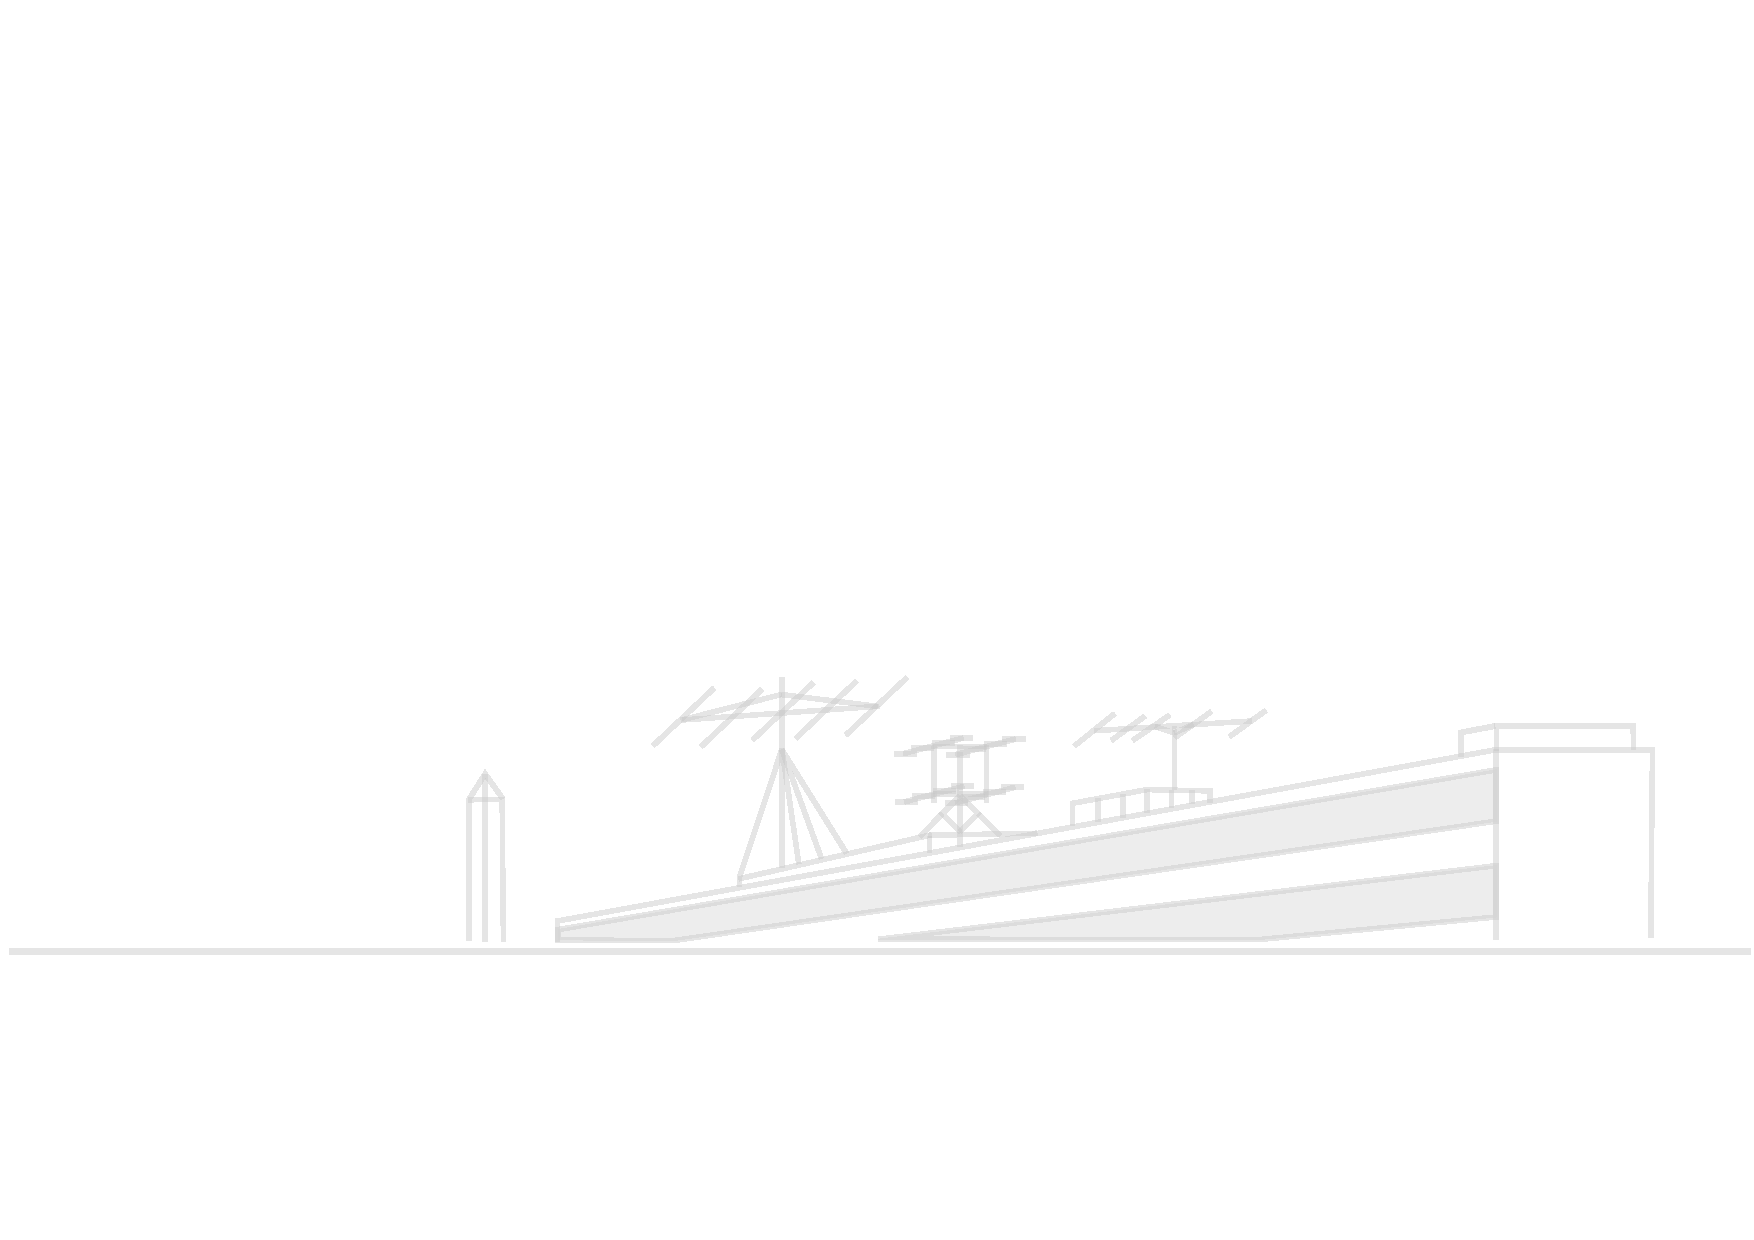
\includegraphics[width=17.8cm]{texdata/dk0tu_rooftop_background.pdf}
}

% Foliennummer einfügen
\setbeamertemplate{footline}[frame number]
%\setbeamertemplate{footline}{}

% Ändere das Zeichen vor jedem item
%\setbeamertemplate{itemize item}{\color{craneorange}$\blacktriangleright$}
%\setbeamertemplate{itemize subitem}{\color{craneorange}$\triangleright$}
%\setbeamertemplate{itemize subsubitem}{\color{craneorange}$\blacktriangleright$}

% Ändert die Blöcke 
\setbeamertemplate{blocks}[rounded][shadow=true]
% default | rounded [shadow=true|false]

%
% Eigene Kommandos
%

% Hack to get natbib and beamer working together. "The beamer user guide suggests
% that only the manual bibliography entry approach is supported"
% on some system it works out of the box, sometimes you need the hack :-(
% so check it --dl7bst
\ifdefined\newblock
    \relax
\else
    \newcommand{\newblock}{}
\fi

% \includedia command to generate png out of a dia file
% NEEDS installed dia and pdflatex option --shell-escape
\newcommand{\includedia}[1]{
    \immediate\write18{/usr/bin/dia #1.dia -e #1_diatmp.png -t png}
}

% RICHIG GROSSER FONT!
\newfont{\bigfont}{cmr10 at 144pt}
\newfont{\smallfont}{cmr10 at 8pt}

% Römische Ziffern
\makeatletter
\newcommand{\rmnum}[1]{\romannumeral #1}
\newcommand{\Rmnum}[1]{\expandafter\@slowromancap\romannumeral #1@}
\makeatother

% Schwarze Überschrift
%\setbeamercolor{frametitle}{fg=black}
%\setbeamercolor{title}{fg=black}

% Item- und Box-Farben
\definecolor{deepBlue}{HTML}{000066}
\setbeamercolor{itemize item}{fg=deepBlue}
\setbeamercolor{itemize subitem}{fg=deepBlue}
\setbeamercolor{description item}{fg=deepBlue}
\setbeamercolor{block title}{fg=deepBlue!100, bg=blue!15}
\setbeamercolor{block body}{fg=black, bg=blue!5}
\setbeamercolor{block title alerted}{fg=deepBlue, bg=red!75}
\setbeamercolor{block body alerted}{fg=black, bg=red!15}
\setbeamercolor*{block title example}{fg=blue!50, bg=blue!10}
\setbeamercolor*{block body example}{fg= blue, bg=blue!5}

%\setbeamercolor{section in head/foot}{parent=palette primary}
%\setbeamercolor{subsection in head/foot}{parent=palette secondary}
%\setbeamercolor{sidebar}{fg=darkblue,bg=yellow!90!orange}
%\setbeamercolor{title in sidebar}{fg=darkblue}
%\setbeamercolor{author in sidebar}{fg=darkblue}
%\setbeamercolor{section in sidebar}{fg=darkblue!10!black}
%\setbeamercolor{subsection in sidebar}{fg=darkblue!50!black}

% Titlepage Infos
\title{AFu-Kurs nach DJ4UF}
\author[DKØTU]{DKØTU\\ \footnotesize{Amateurfunkgruppe der TU Berlin}}
\institute[DKØTU]{\url{http://www.dk0tu.de} }

% PDF-Eigenschaften
\subject{DK0TU-Amateurfunkkurs nach DJ4UF}
\keywords{Amateurfunk Kurs HAM Radio Course CC-BY-NC-SA OpenSource TU Berlin DK0TU}

\subtitle{Technik Klasse E 10: \\
          Dezibel, Dämpfung \& Kabel \\[2em]}
\date{Stand 25.09.2017}
 \begin{document}

\begin{frame}
    \titlepage
    \vfill
    \begin{center}
        \ccbyncsaeu\\
        {\tiny This work is licensed under the \em{Creative Commons Attribution-NonCommercial-ShareAlike 3.0 License}.}\\[0.5ex]
         \tiny Amateurfunkgruppe der Technische Universität Berlin (AfuTUB), DKØTU
         %\includegraphics[scale=0.5]{img/DK0TU_Logo.pdf}
    \end{center}
\end{frame}


\newcommand{\amplifytriangle}{% 
  \tikz{%
    \draw[very thick, fill=blue!60] (0,2) node {}
                                 -- (0,0) node {}
                                 -- (2,1) node[anchor=east,inner sep=2pc] {\Huge{$\times$}}
                                 -- cycle;
  }
}


\section*{Dezibel}

\begin{frame}
  \frametitle{Einschub: Dezibel einfach erklärt}

  \only<1>{%
    \begin{block}{Große und kleine Leistungen}
      Wir haben es im Amateurfunk mit großen und kleinen Leistungen zu tun.
    \end{block}
  }
  \only<2>{%
    \begin{block}{Nullen zählen}
      Zählen wir die Nullen (und nennen das Ergebnis ``Bel'', nach Alexander Graham Bell).
    \end{block}
  }
  \only<3>{%
    \begin{block}{dBm = Dezibel bezogen auf mW}
      Die Bel-Zahl mit 10 malgenommen gibt ``Dezibel'' dB.
    \end{block}
  }
  \only<4>{%
    \begin{block}{dbW = Dezibel bezogen auf W}
      Man kann auch Nullen von Watt-Zahlen zählen. Logischer, aber unüblicher.
    \end{block}
  }
  \only<5>{%
    \begin{block}{``log'' ist die ``Bel''-Taste des Taschenrechners}
      Da wir uns nicht für Bel, sondern für dB interessieren: Noch mit 10 malnehmen.
    \end{block}
  }


  \begin{center}
    \begin{tabular}{p{12pc}|rrr}
      \textbf{Was} & \textbf{Leistung in \only<1-3,5>{m}W} & \only<2-5>{\textbf{Bel}} & \only<3,5>{\textbf{dBm}}\only<4>{\textbf{dbW}} \\ \hline
      effektive Leistung EME-Station & \only<1-3,5>{100\,000\,000}\only<4>{100\,000} & \only<2-3,5>{8}\only<4>{5} & \only<3,5>{80}\only<4>{50} \\
      Standard-Transceiver & \only<1-3,5>{100\,000}\only<4>{100} & \only<2-3,5>{5}\only<4>{2} & \only<3,5>{50}\only<4>{20} \\
      kleine Handfunke & \only<1-3,5>{1\,000}\only<4>{1} & \only<2-3,5>{3}\only<4>{0} & \only<3,5>{30}\only<4>{0} \\
      Lautsprechersignal (Zimmerlautstärke) & \only<1-3,5>{100}\only<4>{0,4} & \only<2-3,5>{2}\only<4>{-1} & \only<3,5>{20}\only<4>{-10} \\
      Kopfhörersignal & \only<1-3,5>{1}\only<4>{0,001} & \only<2-3,5>{0}\only<4>{-3} & \only<3,5>{0}\only<4>{-30} \\
      Lautes KW-Signal & \only<1-3,5>{0,000\,001}\only<4>{0,000\,000\,001} & \only<2-3,5>{-6}\only<4>{-9} & \only<3,5>{-60}\only<4>{-90} \\
      Leises KW-Signal (Antenneneingang RX) & \only<1-3,5>{0,000\,000\,000\,001}\only<4>{0,000\,000\,000\,000\,001} & \only<2-3,5>{-12}\only<4>{-15} & \only<3,5>{-120}\only<4>{-150} \\ \hline
    \end{tabular}
  \end{center}

  \only<1>{Wer mit diesen Zahlen umgeht, fängt automatisch an, die Nullen zu zählen.}
  \only<2>{Von ``mW'' als Basis auszugehen ist willkürlich, aber in der Funktechnik üblich.}
  \only<3>{Man schreibt hinter dem ``dB'' noch ein ``m'', wenn man die Nullen von mW-Zahlen zählt.}
  \only<4>{Man schreibt hinter dem ``dB'' noch ein ``W'', wenn man Nullen von W-Zahlen zählt.}

\end{frame}

\section*{Dämpfung}

\begin{frame}
  \frametitle{Bei Verstärkungen haben wir dasselbe Problem mit vielen Nullen}

  \begin{block}{Empfänger}
    Eingangssignal: 0,000\,000\,000\,001 mW
    Ausgangssignal: 100mW

    Benötigte Verstärkung: 100\,000\,000\,000\,000.
  \end{block}

  \begin{block}{Sender}
    Frequenzerzeugende Stufe (Oszillator): 10 mW
    Ausgangssignal: 100\,000 mW

    Benötigte Verstärkung: 10\,000.
  \end{block}

  Die Verstärkung ist der Faktor, mit dem ich das eine Signal multiplizieren muss, um das andere zu erhalten. Sie hat keine Maßeinheit.
\end{frame}

\begin{frame}
  \frametitle{Mit dB wird's einfacher!}

  \begin{block}{Empfänger}
    Eingangssignal: 0,000\,000\,000\,001 mW = -120 dBm
    Ausgangssignal: 100 mW = 20 dBm

    Benötigte Verstärkung: 100\,000\,000\,000\,000 = 140 dB.
  \end{block}

  \begin{block}{Sender}
    Frequenzerzeugende Stufe (Oszillator): 10 mW = 10 dBm
    Ausgangssignal: 100\,000 mW = 50 dBm

    Benötigte Verstärkung: 10\,000 = 40 dB
    Verstärkung in dB ohne ``m''.
  \end{block}

  Verstärkung in dB lässt sich durch Subtraktion ausrechnen:\\
  $50 - 10 = 40$\\
  $20 - (-120) = 140$
\end{frame}

\begin{frame}
  \frametitle{Dämpfungsfaktor}
  \begin{center}
    \begin{minipage}{0.3\textwidth}
      \huge{$ D = \cfrac{P_{in}}{P_{out}}$}
    \end{minipage}
    \begin{minipage}{0.6\textwidth}
      \begin{itemize}
        \item Dämpfungsfaktor D gibt Verhältnis zwischen Eingangsleistung $P_{in}$
          und der Ausgangsleistung $P_{out}$.
      \end{itemize}
    \end{minipage}
    \vspace{1cm}
    \begin{figure}
      % FIXME Uebertragungsstrecke von Martin war totaler Quatsch - korrigiert wie im Moltrecht, muss aber neu
      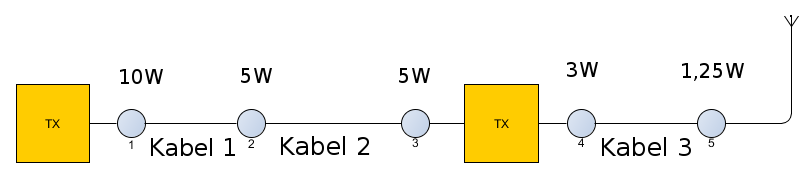
\includegraphics[width=\textwidth,height=.4\textheight,keepaspectratio]{e10/ubertragung.png}
      \caption{Übertragungswege einer Funkstation}
    \end{figure}
  \end{center}
\end{frame}

\begin{frame}
  \frametitle{Dämpfungsmaß dB}
  \begin{itemize}
    \item Dämpfungsmaß ist die Logarithmierung des Dämpfungsfaktors
    \item Einheit Bel $\rightarrow dB$
    \item durch Logarithmusgesetze: Multiplikation $\rightarrow$ Addition
  \end{itemize}
  \vspace{0.5cm}
  \begin{block}{Dämpfungsmaß}
    \Huge{$a = 10 \cdot log(\frac{P_{in}}{P_{out}})$ dB}
  \end{block}
\end{frame}

\begin{frame}
  \frametitle{Verstärkung in dB}
  \begin{itemize}
    \item generell wird eher mit Verstärkung und nicht mit Dämpfung gerechnet
    \item Dämpfung ist eine negative Verstärkung
  \end{itemize}
  \vspace{1cm}
  \begin{block}{Verstärkung}
    \Huge{$g = 10 \cdot log(\frac{P_{out}}{P_{in}})$ dB}
  \end{block}
\end{frame}

\begin{frame}
  \frametitle{Verstärkungen verketten}
  \begin{center}
    \begin{tabular}{ccc}
      \amplifytriangle & \amplifytriangle& \amplifytriangle \\
      $\times 100$ & $\times 10$ & $\times 1000$ \\
      \multicolumn{3}{c}{Gesamtverstärkung: 1\,000\,000 (multipliziert)}\\ \\
      $20 dB$ & $10 dB$ & $30 dB$ \\
      \multicolumn{3}{c}{Gesamtverstärkung: 60dB (addiert)}\\
    \end{tabular}
  \end{center}
\end{frame}

\begin{frame}
  \frametitle{``Krumme'' Bel-Werte\footnote{für mathematisch Interessierte}}

  \begin{itemize}
    \item 10 Verstärker je $\times 2$ ergeben zusammen $1024 \approx 30dB$.
    \item Also muss die passende dB-Zahl für 2 etwa 3dB sein.\\[1.5em]
    \item Zwei Verstärker je $x\sqrt{10}$ ergeben zusammen 10, also genau 10 dB.
    \item Die passende dB-Zahl für $\sqrt{10}$ muss deshalb \emph{genau} 5 dB sein.\\[1.5em]
    \item Analog $\sqrt{\sqrt{10}} \Rightarrow 2,5dB$, $\sqrt{\sqrt{\sqrt{10}}} \Rightarrow 1,25dB$ und so weiter.\\[1.5em]
    \item Man kann auf dieser Basis tatsächlich ein Programm schreiben, das dB-Werte ausrechnet. Taschenrechner nutzen geschicktere Methoden, die aber nicht so leicht zu erklären sind.
  \end{itemize}
\end{frame}



\begin{frame}
  \frametitle{Verstärkung in dB}
  \begin{columns}
    \column{.5\textwidth}
    \begin{center}
      \begin{Large}
        \begin{tabular}{c|c}
          dB & $\approx$ Leistungsfaktor \\
          \hline \hline
          0    & 1                  \\
          1,5  & $\sqrt{2}$ = 1,41  \\
          2,15 & 1,64               \\
          3    & 2                  \\
          5    & $\sqrt{10}$ = 3,16 \\
          6    & 4                  \\
          10   & 10                 \\
          20   & 100                \\
        \end{tabular}
      \end{Large}
    \end{center}
    \column{.5\textwidth}
    \begin{block}{Taschenrechner}
      Verstärkung $\rightarrow$ $log$-Taste $\rightarrow$ $\times 10$\\[1.5em]
      dB $\rightarrow$ $\div 10$ $\rightarrow$ $10^x$-Taste
    \end{block}
  \end{columns}
\end{frame}

\begin{frame}
  \frametitle{Spannungs\-dämpfungs\-maß}
  \begin{block}{Spannungsdämpfungsmaß}
    \Huge{$a_{U} = 20 \cdot log(\frac{U_{1}}{U_{2}})$ dB}
  \end{block}
  \vspace{2cm}
  Wird in der A-Technik näher erläutert.
\end{frame}

\begin{frame}
  \frametitle{Spannungsfaktor \& Leistungsfaktor}
  \begin{center}
    \begin{Huge}
      \begin{minipage}{0.3\textwidth}
        \begin{tabular}{|c|c|}
          \hline
          \textbf{dB} & $a_{U}$ \\
          \hline \hline
          \alert{6dB}  & \alert{2}  \\ \hline
          12dB & 4  \\ \hline
          \alert{20dB} & \alert{10} \\ \hline
        \end{tabular}
      \end{minipage}
      \hspace{2cm}
      \begin{minipage}{0.3\textwidth}
        \begin{tabular}{|c|c|}
          \hline
          \textbf{dB} & $a_{P}$ \\
          \hline \hline
          \alert{3dB}  & \alert{2}  \\ \hline
          6dB  & 4  \\ \hline
          \alert{10dB} & \alert{10} \\ \hline
        \end{tabular}
      \end{minipage}
    \end{Huge}
  \end{center}
\end{frame}

\section*{S-Stufen}
\begin{frame}
  \frametitle{S-Stufen}
  \begin{center}
    \begin{figure}
      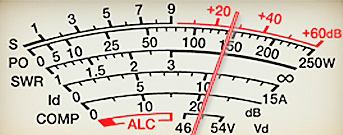
\includegraphics[width=\textwidth,height=.4\textheight,keepaspectratio]{e10/S-Meter.jpg}
      \attribcaption{S-Meter}{Cqdx}{https://commons.wikimedia.org/wiki/File:S-Meter.jpg}{\ccbysa}
    \end{figure}
    \begin{itemize}
      \item eine S-Stufe entspricht $6 dB \rightarrow$ Faktor?
      \item Wird beim RST-System verwendet
      \item gibt einen bestimmten Spannungswert an einem $50\Omega$ Widerstand an
      \item Kurzwelle: S9 = $50\mu V$ bei $50\Omega$
      \item UKW: S9 = $5\mu V$ bei $50\Omega$
    \end{itemize}
  \end{center}
\end{frame}

\section{Pegel}

\begin{frame}
  \frametitle{Pegel}

    \begin{itemize}
      \item Pegel ist auf einen Grundwert $P_0$ bezogen
      \item Grundwert wird auch Normal oder Nullwert genannt
    \end{itemize}

    \begin{block}{Leistungspegel}
      \centering \Large $L_P = 10 lg \frac{P}{P_0} dB$\alert{x}
    \end{block}

  \begin{center}
    \begin{minipage}{0.3\textwidth}
      \begin{tabular}{|c|c|}
        \hline
        $dBm$ & $P_0 = 1 mW$ \\
        \hline \hline
        20dBm  & 100mW  \\ \hline
        10dBm  & 10mW   \\ \hline
        0dBm   & 1mW    \\ \hline
        -10dBm & 0,1mW  \\ \hline
      \end{tabular}
    \end{minipage}
    \hspace{2cm}
    \begin{minipage}{0.3\textwidth}
      \begin{tabular}{|c|c|}
        \hline
        $dBW$ & $P_0 = 1 W$ \\
        \hline \hline
        20dBW  & 100W  \\ \hline
        10dBW  & 10W   \\ \hline
        0dBW   & 1W    \\ \hline
        -10dBW & 0,1W  \\ \hline
      \end{tabular}
    \end{minipage}
    \vspace{0.5cm}
  \end{center}
\end{frame}


\section*{Leiter}
\begin{frame}
  \frametitle{Hochfrequenzleitungen}
  %FIXME Erläuterungen der Bilder fehlen
  \begin{center}
    \begin{columns}
      \column{.55\textwidth}
      \begin{center}
        \begin{figure}
          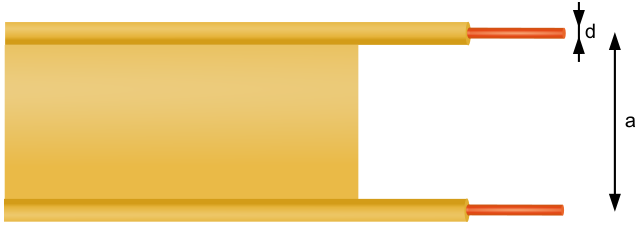
\includegraphics[width=1\textwidth,height=.5\textwidth,keepaspectratio]{e10/parallel.png}
          \attribcaption{Paralleldrahtleitung}{SpinningSpark, Inductiveload, Wdwd}
                        {https://commons.wikimedia.org/wiki/File:Twin-lead_cable_dimension.svg}{\ccbysa}
        \end{figure}
      \end{center}
      \column{.4\textwidth}
      \begin{center}
        \begin{figure}
          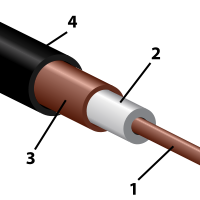
\includegraphics[width=1\textwidth,height=.5\textwidth,keepaspectratio]{e10/coax.png}
          \attribcaption{Koaxialkabel}{Tkgd2007, Fleshgrinder}
                  {https://commons.wikimedia.org/wiki/File:Coaxial_cable_cutaway_new.svg}{\ccby}
        \end{figure}
      \end{center}
    \end{columns}
  \end{center}
\end{frame}

\begin{frame}
  \frametitle{Hochfrequenzleitungen}
  \begin{center}
    \begin{figure}
      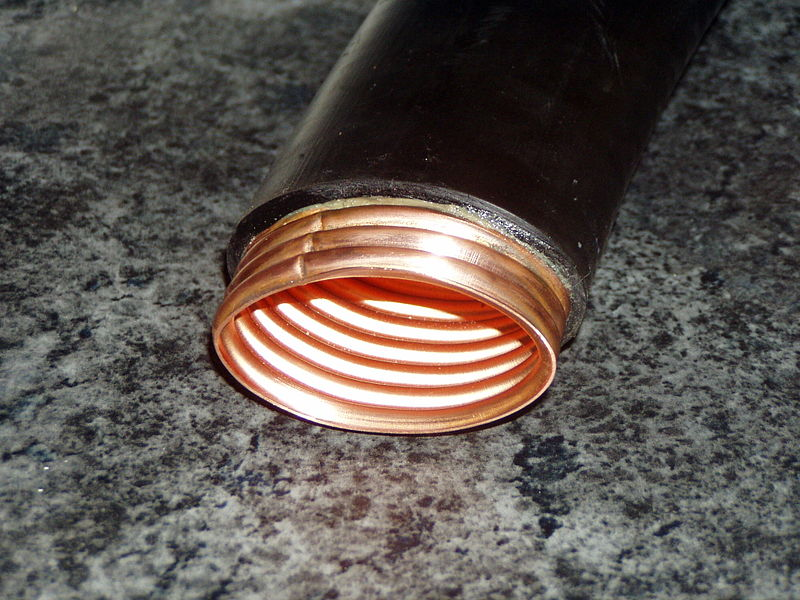
\includegraphics[width=1\textwidth,height=.7\textheight,keepaspectratio]{e10/hohl.jpg}
      \attribcaption{Hohlleiter}{Averse}{https://commons.wikimedia.org/wiki/File:Elli_holl.jpg}{\ccbysa}
    \end{figure}
    %\end{minipage}
\end{center}
\end{frame}

\subsection*{Wellen\-widerstand}
\begin{frame}
  \frametitle{Wellenwiderstand}
  \begin{figure}
    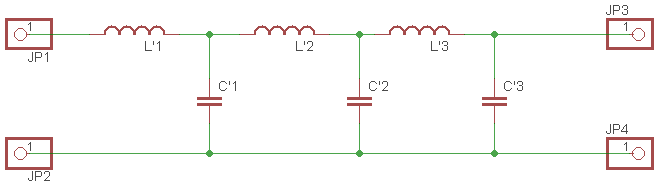
\includegraphics[width=1\textwidth,height=.3\textheight,keepaspectratio]{e10/wellenesb.png}
    \caption{Ersatzschaltbild}
  \end{figure}
  %\vspace{1cm}\\
  \begin{figure}
    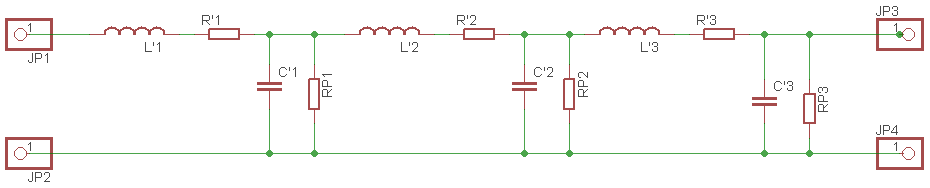
\includegraphics[width=1\textwidth,height=.3\textheight,keepaspectratio]{e10/wellenesbex.png}
    \caption{Genaues Ersatzschaltbild eines Koxialkabels}
  \end{figure}
\end{frame}

\begin{frame}
  \frametitle{Wellenwiderstand}
  \begin{block}{Wellenwiderstand}
    \Huge{$Z_W = \sqrt{\frac{L'}{C'}}$}
  \end{block}
  \begin{itemize}
    \normalsize \item Paralleldrahtleitungen: $Z_W = 150 \Omega \cdots 600 \Omega$
    \item Koaxialleitungen: $Z_W =  50 \Omega \cdots 95 \Omega$ -- verbreitet:
      \begin{itemize}
        \item $50 \Omega$ !
        \item $60 \Omega$
        \item $75 \Omega$
      \end{itemize}
    \item Wellenwiderstand entspricht dem Abschlusswiderstand einer Leitung, bei
      dem keine stehenden Wellen auftreten $\rightarrow SWR$
  \end{itemize}
\end{frame}

\begin{frame}
  \frametitle{Dämpfungsberechnung}
  \begin{Large}
    Formelsammlung, Diagramm auf der letzten Seite.
  \end{Large}
\end{frame}

\begin{frame}
  \frametitle{Gemeinsame Rechnung (optional)}
  \begin{exampleblock}{Übung 1}
    \begin{description}
      \item[Kabel] RG58
      \item[Länge] 10 m
      \item[Frequenz] 145 MHz
    \end{description}
  \end{exampleblock}
\end{frame}

\begin{frame}
  \frametitle{Gemeinsame Rechnung (optional)}
  \begin{exampleblock}{Übung 2}
    \begin{description}
      \item[Kabel] Aircell7
      \item[Länge] 40 m
      \item[Frequenz] 29 MHz
    \end{description}
  \end{exampleblock}
\end{frame}

\begin{frame}
  \frametitle{Gemeinsame Rechnung (optional)}
  \begin{exampleblock}{Übung 3}
    \begin{description}
      \item[Kabel] RG174
      \item[Länge] 5 m
      \item[Frequenz] 1296 MHz
    \end{description}
  \end{exampleblock}
\end{frame}


\subsection*{Anpassung}
\begin{frame}
  \frametitle{Anpassung}
  \begin{center}
    \begin{figure}
      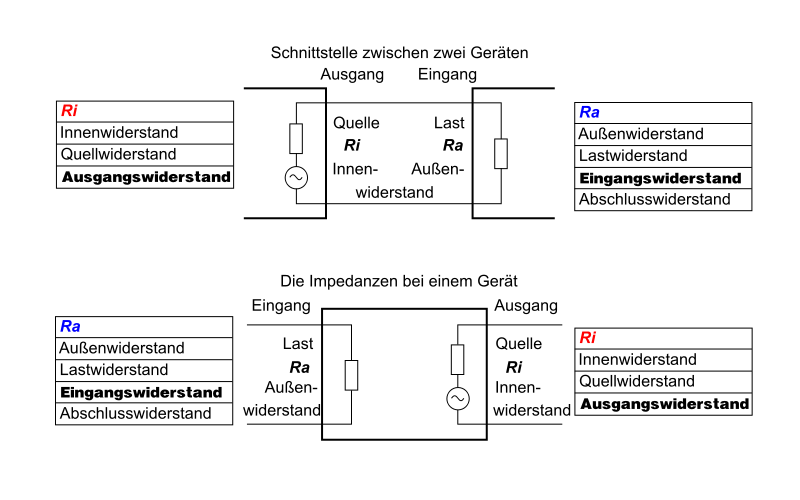
\includegraphics[width=1\textwidth,height=.7\textheight,keepaspectratio]{e10/Anpassung.png}
      \attribcaption{Anpassung}{Frank Murmann}
                    {https://commons.wikimedia.org/wiki/File:EingangswiderstandAusgangswiderstandA.svg}{\ccpd}
    \end{figure}
  \end{center}
\end{frame}

\begin{frame}
  \frametitle{Stehwellenverhältnis}
  \begin{itemize}
    \item ist ein Maß für die Anpassung
    \item ist das Verhältnis von vorlaufender zu zurücklaufender Welle
  \end{itemize}
  \begin{block}{}
    \centering $SWR = \cfrac{u_{vorlaufend}+u_{ruecklaufend}}{u_{vorlaufend}-u_{ruecklaufend}}$
  \end{block}
  \begin{center}
    \begin{figure}
      %\animategraphics[loop,width=\textwidth,height=0.3\textheight,keepaspectratio,controls]{10}{e10/Stehwelle-}{0}{80}
      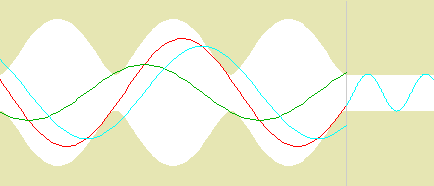
\includegraphics[width=\textwidth,height=0.3\textheight,keepaspectratio]{e10/Stehwelle-10.png}
      \attribcaption{\centering Stehwelle mit SWR 4 \newline
           {\footnotesize (blau: vorlaufende Welle, grün: reflektierte Welle,
           rot: Überlagerung)}}{Pyrometer}
           {https://commons.wikimedia.org/wiki/File:Standing_wave_SWR_4_(forward,_reflected)_open.gif}{\cczero}
    \end{figure}
  \end{center}
\end{frame}

\begin{frame}
  \frametitle{Symmetrierung}
  \begin{minipage}{0.3\textwidth}
    \begin{figure}
      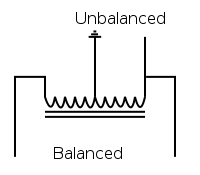
\includegraphics[width=1\textwidth,height=.8\textheight,keepaspectratio]{e10/balun.png}
      \attribcaption{Balun}{Wolfmankurd}{https://commons.wikimedia.org/wiki/File:Cdbalun2.svg}{\ccbysa}
    \end{figure}

  \end{minipage}
  \begin{minipage}{0.6\textwidth}
    \begin{itemize}
      \item Wird bei Verbindungen zwischen symmetrischen und unsymmetrischen Punkten verwendet
      \item Koaxialkabel ist unsymmetrisch
      \item Paralleldraht ist symmetrisch
      \item Alle Dipole sind symmetrisch
      \item Alle Antennen die gegen Erde erregt werden sind unsymmetrisch
    \end{itemize}
  \end{minipage}
\end{frame}

\section*{Stecker und Adapter}
\begin{frame}
  \frametitle{Stecker und Adapter}
  \begin{center}
    \begin{figure}
      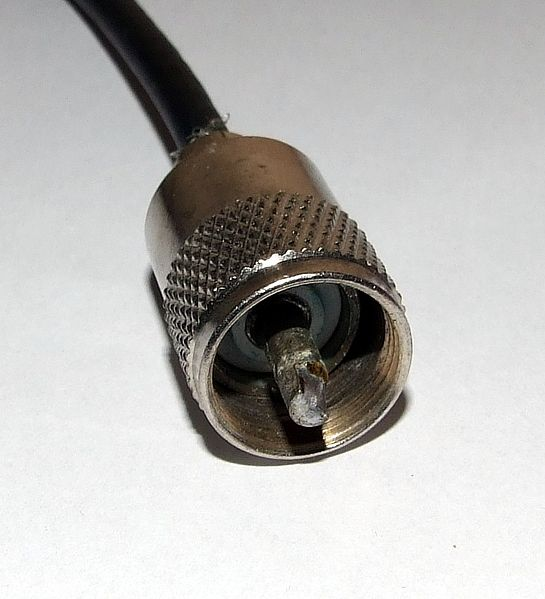
\includegraphics[width=.6\textwidth,height=.55\textheight,keepaspectratio]{e10/pl.jpg}
      \attribcaption{UHF- oder PL-Stecker}{Appaloosa}
                    {https://commons.wikimedia.org/wiki/File:UHF_PL_Connector.jpg}{\ccbysa}
    \end{figure}
    \begin{itemize}
      \item UHF im Namen, aber ungeeignet dafür
      \item Kurzwelle, auch 2-Meter-Band
      \item ``geschirmter Bananenstecker''
    \end{itemize}
  \end{center}
\end{frame}

\begin{frame}
  \frametitle{Stecker und Adapter}
  \begin{center}
    \begin{figure}
      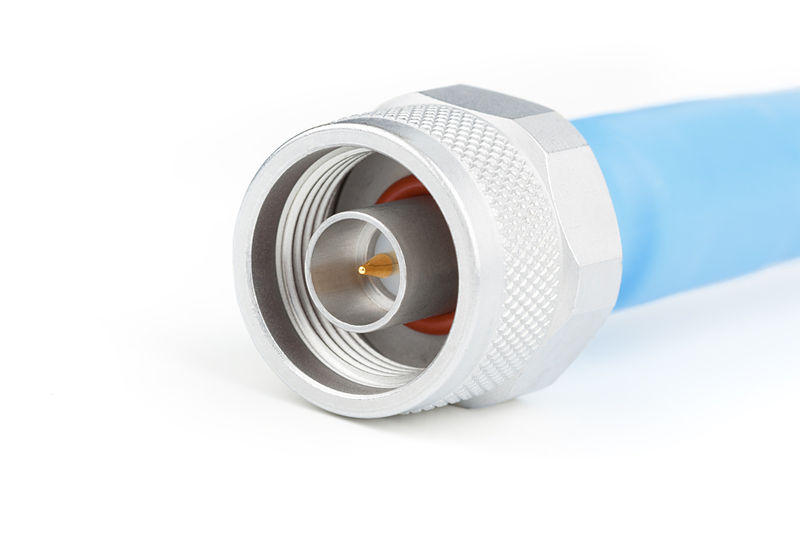
\includegraphics[width=.6\textwidth,height=.6\textheight,keepaspectratio]{e10/n.jpg}
      \attribcaption{N-Stecker}{Swift.Hg}
                    {https://commons.wikimedia.org/wiki/File:Male_type_N_connector.jpg}{\ccbysa}
    \end{figure}
    \begin{itemize}
      \item N
      \item HF \dots 70-cm und höher
    \end{itemize}
  \end{center}
\end{frame}

\begin{frame}
  \frametitle{Stecker und Adapter}
  \begin{center}
    \begin{figure}
      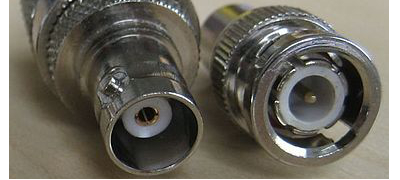
\includegraphics[width=.6\textwidth,height=.7\textheight,keepaspectratio]{e10/bnc.jpg}
      \attribcaption{BNC-Stecker und -Buchse}{Kaback}
                    {https://commons.wikimedia.org/wiki/File:BNC_50_75_Ohm.jpg}{\ccbysa}
    \end{figure}
    \begin{itemize}
      \item BNC
      \item HF \dots 70-cm und höher
    \end{itemize}

  \end{center}
\end{frame}

\begin{frame}
  \frametitle{Stecker und Adapter}
  \begin{center}
    \begin{figure}
      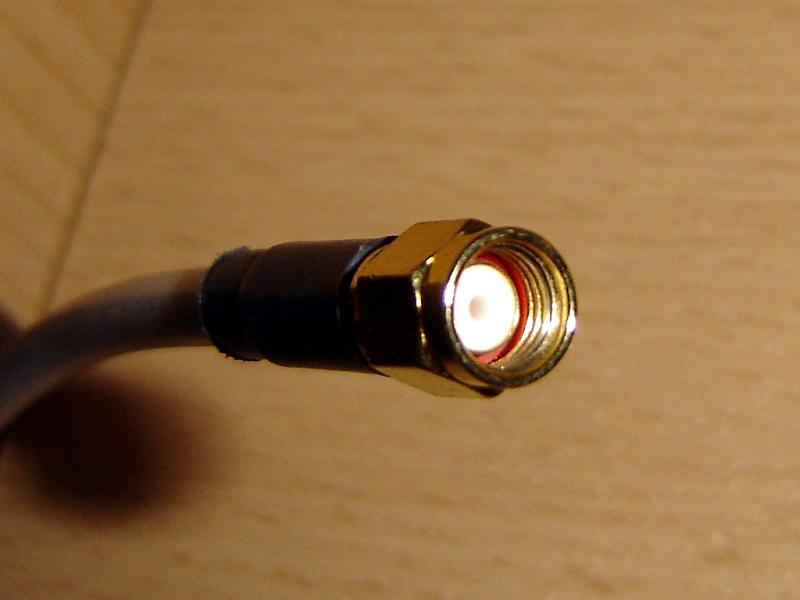
\includegraphics[width=.6\textwidth,height=.6\textheight,keepaspectratio]{e10/sma.jpg}
      \attribcaption{RP-SMA-Stecker}{Peter Trieb}
                    {https://commons.wikimedia.org/wiki/File:BNC_50_75_Ohm.jpg}{\ccpd}
    \end{figure}
    \begin{itemize}
      \item SMA
      \item VHF-/UHF-Handfunkgeräte
    \end{itemize}
  \end{center}
\end{frame}

\section*{Referenzen}
\begin{frame}
  \frametitle{Referenzen/Links}

    \footnotesize
    \begin{itemize}
      \item Moltrecht E 10: \\
        \url{https://www.darc.de/der-club/referate/ajw/lehrgang-te/e10/}
    \end{itemize}

\end{frame}

% Hier könnte noch eine Kontaktfolie stehen

\end{document}

